\def\year{2019}\relax
%File: formatting-instruction.tex
\documentclass[letterpaper]{article} %DO NOT CHANGE THIS
\usepackage{aaai19}  %Required
\usepackage{times}  %Required
\usepackage{helvet}  %Required
\usepackage{courier}  %Required
\usepackage{url}  %Required
\usepackage{graphicx}  %Required
\usepackage{amssymb}
\usepackage{amsmath}
\usepackage[sort&compress,square,comma,authoryear]{natbib}

\usepackage{amsfonts}
\usepackage{amssymb}
\usepackage{amsthm}
\usepackage{bbm}
\usepackage{latexsym}
\usepackage{mathtools}

\usepackage{algorithm}
\usepackage{algorithmic}


\frenchspacing  %Required
\setlength{\pdfpagewidth}{8.5in}  %Required
\setlength{\pdfpageheight}{11in}  %Required


%PDF Info Is Required:
  \pdfinfo{
/Title (2019 Formatting Instructions for Authors Using LaTeX)
/Author (AAAI Press Staff)}
\setcounter{secnumdepth}{0}  

\DeclareMathOperator*{\argmin}{argmin}
\DeclareMathOperator*{\argmax}{argmax}

\newcommand{\km}[1]{{\color{red} #1}} %red comments: Karsten
\newcommand{\wb}[1]{{\color{blue} #1}} %blue comments: Walter

\begin{document}
% The file aaai.sty is the style file for AAAI Press 
% proceedings, working notes, and technical reports.
%
\title{Facility Location Utility for Uncovering Unknown Unknowns}
\author{Karsten Maurer$^1$ \hspace{.2in} Walter Bennette$^2$\\
$^1$Miami University Department of Statistics - maurerkt@miamioh.edu\\ 
$^2$Air Force Research Lab Information Directorate - walter.bennette.1@us.af.mil \\
}

\maketitle
\begin{abstract}
AAAI creates proceedings, working notes, and technical reports directly from electronic source furnished by the authors. To ensure that all papers in the publication have a uniform appearance, authors must adhere to the following instructions. 
\end{abstract}

\section{Introduction}

Techniques such as active learning \citep{Settles2010} and domain adaptation \citep{Patel2014} can be used to create machine learning classifiers when large labeled datasets are not available for a specific task.  For example, the black box classifiers made available through many online services (list services) require no training data and can be thought of as a kind of domain adaptation.  However, with limited amounts of labeled data, users may not be able to properly evaluate a model, and are left hoping the model will be useful for their intended task.  In this paper we build upon previous work to develop an interactive method to help evaluate classifiers in the absence of labeled data.  Specifically, we develop an interactive method to uncover unknown unknowns \citep{Attenberg2015}: instances for which a classifier is confident in its prediction, but is wrong.  

Intuitive methods can be used to evaluate the performance of a model in the absence of labeled data.  Given a labeling budget one could sample instances following an experimental design, sample instances with the lowest classifier confidence, or sample instances identified as informative to the classifier through active learning strategies.  These methods could provide a sense of a model's performance but will potentially miss high confidence mistakes, referred to as \textit{unknown unknowns}.     

Unknown unknowns can be thought of as blind spots to a classification model, and can be caused by dataset bias during training, domain shift during use, lack of model expressibility, and other causes of poor model fit.  From the viewpoint of a rational actor, unknown unknowns represent costly mistakes because minimal risk mitigation strategies will have been deployed for these high confidence predictions.  The discovery of unknown unknowns may allow new mitigation strategies to be formulated \citep{Nushi2016a}.  Additionally, as enumerated in \citep{Bansal2018}, finding unknown unknowns is valuable to understand classifier limitations and prevent attacks (stole this hard) what do you mean by attacks?. 

\citet{Attenberg2015} gamified the search for unknown unknowns and relied on human oracles to discover misclassified instances. A utility-based search algorithm for discovering unknown unknowns was then proposed by \citet{Lakkaraju2016} and expanded upon by \citet{Bansal2018}. \citet{Lakkaraju2016} uses a utility model that simply counts the number of discovered unknown unknowns and searches using multi-armed bandits. \citet{Bansal2018} argued that this unit utility model motivates the discovery of very similar unknown unknowns. To fix this problem they proposed an adaptive coverage-based utility model that attempts to encourage the discovery of unknown unknowns throughout the feature space, favoring high confidence regions. They then search for unknown unknowns via a greedy algorithm to maximize utility. 

The utility in \citet{Bansal2018} has the form: $$U(Q) = \sum_{x \in \mathbb{X}} c_x \cdot \max_{q \in S} \left\{sim\left(x,q \right) \right\}$$ where $\mathbb{X} \subset \mathbb{R}^p$ is the set of available $p$-dimensional unlabeled test instances, $Q \subset \mathbb{X}$ is the set of instances labeled by an oracle, $S = \left\{x|x \in Q, y_x \neq M(x)\right\}$ is the set of discovered unknowns unknowns for some classifier $M(x):\mathbb{X} \rightarrow class$, $c_x$ is the classifier's confidence in its prediction of $x$, and $sim(x,q)$ is a distance based similarity metric.  The instance $q'$ that maximizes the expected utility increase is greedily selected to be labeled by the oracle $$E\left[U_x\left(Q \cup q'\right)\right] = \hat{\phi}(x) \cdot c_x \cdot \max_{q \in S \cup q'} \left\{sim\left(x,q \right) \right\}$$ where $\hat{\phi}(x) = P\left(y_x \neq M(x) |Q \right)$ is a conditional probability that $x$ is misclassified given the query set.  As previously stated, this method is designed to incentivize a broader search for unknown unknowns and gives higher utility for finding misclassifications in higher confidence regions.  

Unfortunately, the method of \citet{Bansal2018} is consistently outperformed by sequentially querying the instances for which the classifier is most uncertain, as shown in Figure \cite{something}.  We believe this exposes a flaw in the coverage-based utility model.  That is, the coverage-based utility model rewards the discovery of misclassified instances in close proximity to instances for which the classifier has high confidence.  This reward strategy would help find high confidence unknown unknowns if instances with similar model prediction confidence scores were near each other in the feature space, but this does not seem to be the case.




What we find wrong...

\section{Problem Formulation}


\begin{figure}[hbtp]
\centering
  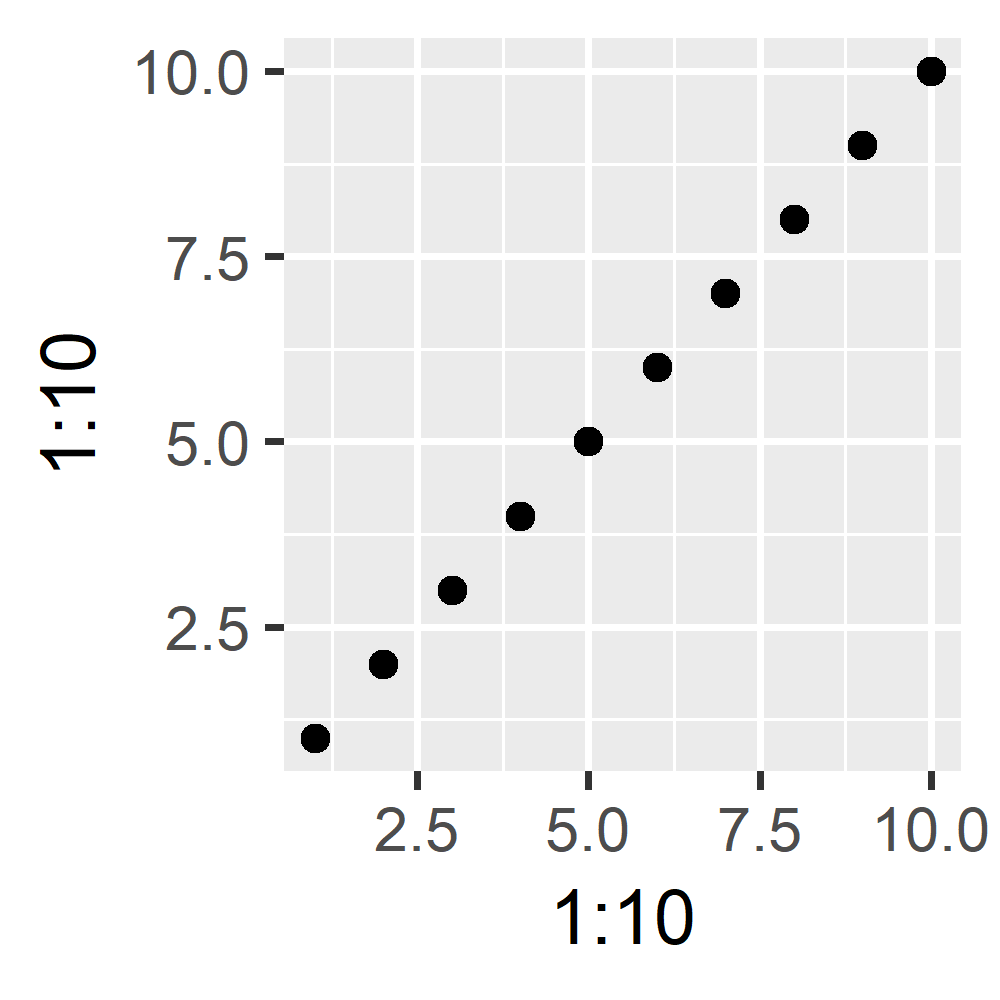
\includegraphics[width=.4\textwidth]{../experimentsAndPlots/demoplot.png}
  \caption{Demo Plot Built in Code Chunk}
  \label{fig:demo}
\end{figure}

\section{Methodology}

$$W(Q) = \sum_{x \in S} r \left(c_x\right) - \frac{1}{n} \sum_{x \in \mathbb{X}} \min_{q \in S}\left(d\left(x,q\right)\right)$$

$r\left(c_x\right) = \log\left(\frac{1}{1-c_x}\right)$


%	FISTA with separation
\begin{algorithm}
	\caption{Greedy Facility Location Search}
	\label{alg:Greedy}
	\begin{algorithmic}
		\STATE {\bfseries Input:} Test set $\mathbb{X}$, prior $\hat{\phi}\left(x|Q=\emptyset\right)$, budget B
		\STATE $Q=\{\}$ \{inputs that have been queried\}
		\STATE $y_Q = \{\}$ \{oracle defined labels\}
		\STATE{\bfseries For: } $b = 1, 2, ..., B$ {\bfseries do:}

		\STATE $q' = \argmax_{q' \not\in Q} E \left[W\left(Q \cup q'\right) \right]$
		
		\STATE $y_{q'} = OracleQuery(q')$
		\STATE $Q \leftarrow Q \cup q'$
		\STATE $S \leftarrow \left\{x | x \in Q \space \text{ and } y_x \neq M(x) \right\}$
		\STATE $b \leftarrow b + 1$
			

		\STATE {\bfseries Return: $Q$ and $y_q$}
	\end{algorithmic}
\end{algorithm}



\section{Experimental Evaluation}



\section{Discussion \& Conclusions}



\newpage
\bibliographystyle{aaai}

\bibliography{library}




\end{document}
